%   ------------------------------------------------------------------------
\FloatBarrier
\subsection{Geração da animação do personagem abrindo a porta}
\label{s.gemini.animacaoAbrirPorta}

Foi tentado criar uma animação do personagem abrindo a porta. Como só era possível anexar uma imagem, a ideia era criar a animação apenas do movimento do personagem, sem a porta realmente presente em cena. 

Diversas tentativas de prompt foram feitas, todas indicando que a porta não deveria aparecer durante o vídeo. Porém, todos os resultados\footnote{\url{https://drive.google.com/drive/folders/1b-mW7EVslZTTQWzP5O5M7vZzSb3UrFpH?usp=sharing}} desenharam a porta a ser aberta, com distintos níveis de precisão do movimento, consistência do personagem e coerência da animação com o estilo. Interessante de se notar, as portas geradas não possuíam nenhuma animação de abertura, apenas sendo deslizadas para o lado até saírem da tela. Analisando esses resultados, foi notado que quando a instrução descrevia com mais detalhes a ação de abrir a porta, mais a IA ficava criativa durante esse movimento, a ponto de gerar ações extras desnecessárias para o personagem. Os testes podem ser consultados nas Figuras \ref{fig:geminiProAbrirPorta1} a \ref{fig:geminiProAbrirPorta5} no Apêndice \ref{ap.telasIA}.

Posteriormente, foi descartada a necessidade dessa animação ser criada, por causa do funcionamento e ambiente do jogo, onde o personagem não iria conseguir interagir com um objeto que está ao lado dele, apenas em frente. Em vez disso, a porta em side view se abre automaticamente quando o sprite do personagem se aproxima, sem nenhuma animação extra do personagem.

Porém, uma das animações geradas apresentou o personagem andando antes de abrir a porta, com um movimento extremamente preciso utilizando a versão final do sprite, como pode ser visto na Figura \ref{fig:geminiProAbrirPortaAndar}. Esse vídeo foi visto como candidato para ser usado na funcionalidade Animação para Animação do Pixel Lab (detalhada na Seção \ref{s.pixelLab.animacao}) com o objetivo de gerar uma animação de caminhada mais consistente.  

\begin{figure}[htbp]
    \centering
    \caption{\small Quadro do personagem andando durante a animação de abrir porta gerada no Gemini Pro}
    \label{fig:geminiProAbrirPortaAndar}
    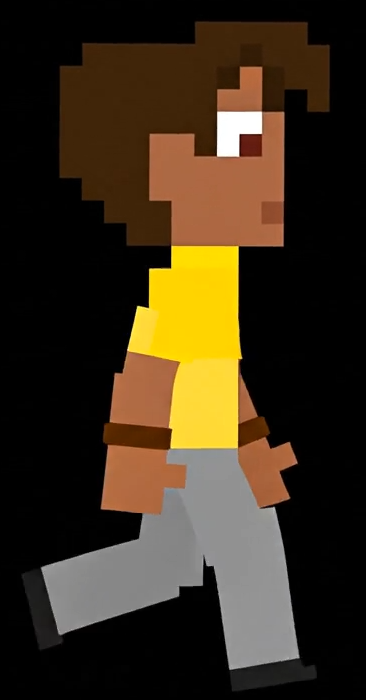
\includegraphics[width=0.2\linewidth]{figs/geminiPro/chat7/andarPreciso.PNG}
    \legend{\small Fonte: Elaborada pela autora, utilizando a ferramenta Gemini Pro.}
\end{figure}

Para isso, foi extraído o sprite sheet do vídeo usando o ezgif (mencionado anteriormente), que depois foi transformado para o padrão pixel perfect através do Pixilart, selecionando apenas o trecho de interesse da animação e removendo o fundo. As Figuras \ref{fig:geminiProAbrirPortaSpriteSheet} a \ref{fig:geminiProAbrirPortaSemFundo} demonstram o processo da transformação do sprite sheet.

\begin{figure}[htbp]
    \centering
    \caption{\small Sprite sheet da animação de abrir porta gerada no Gemini Pro}
    \label{fig:geminiProAbrirPortaSpriteSheet}
    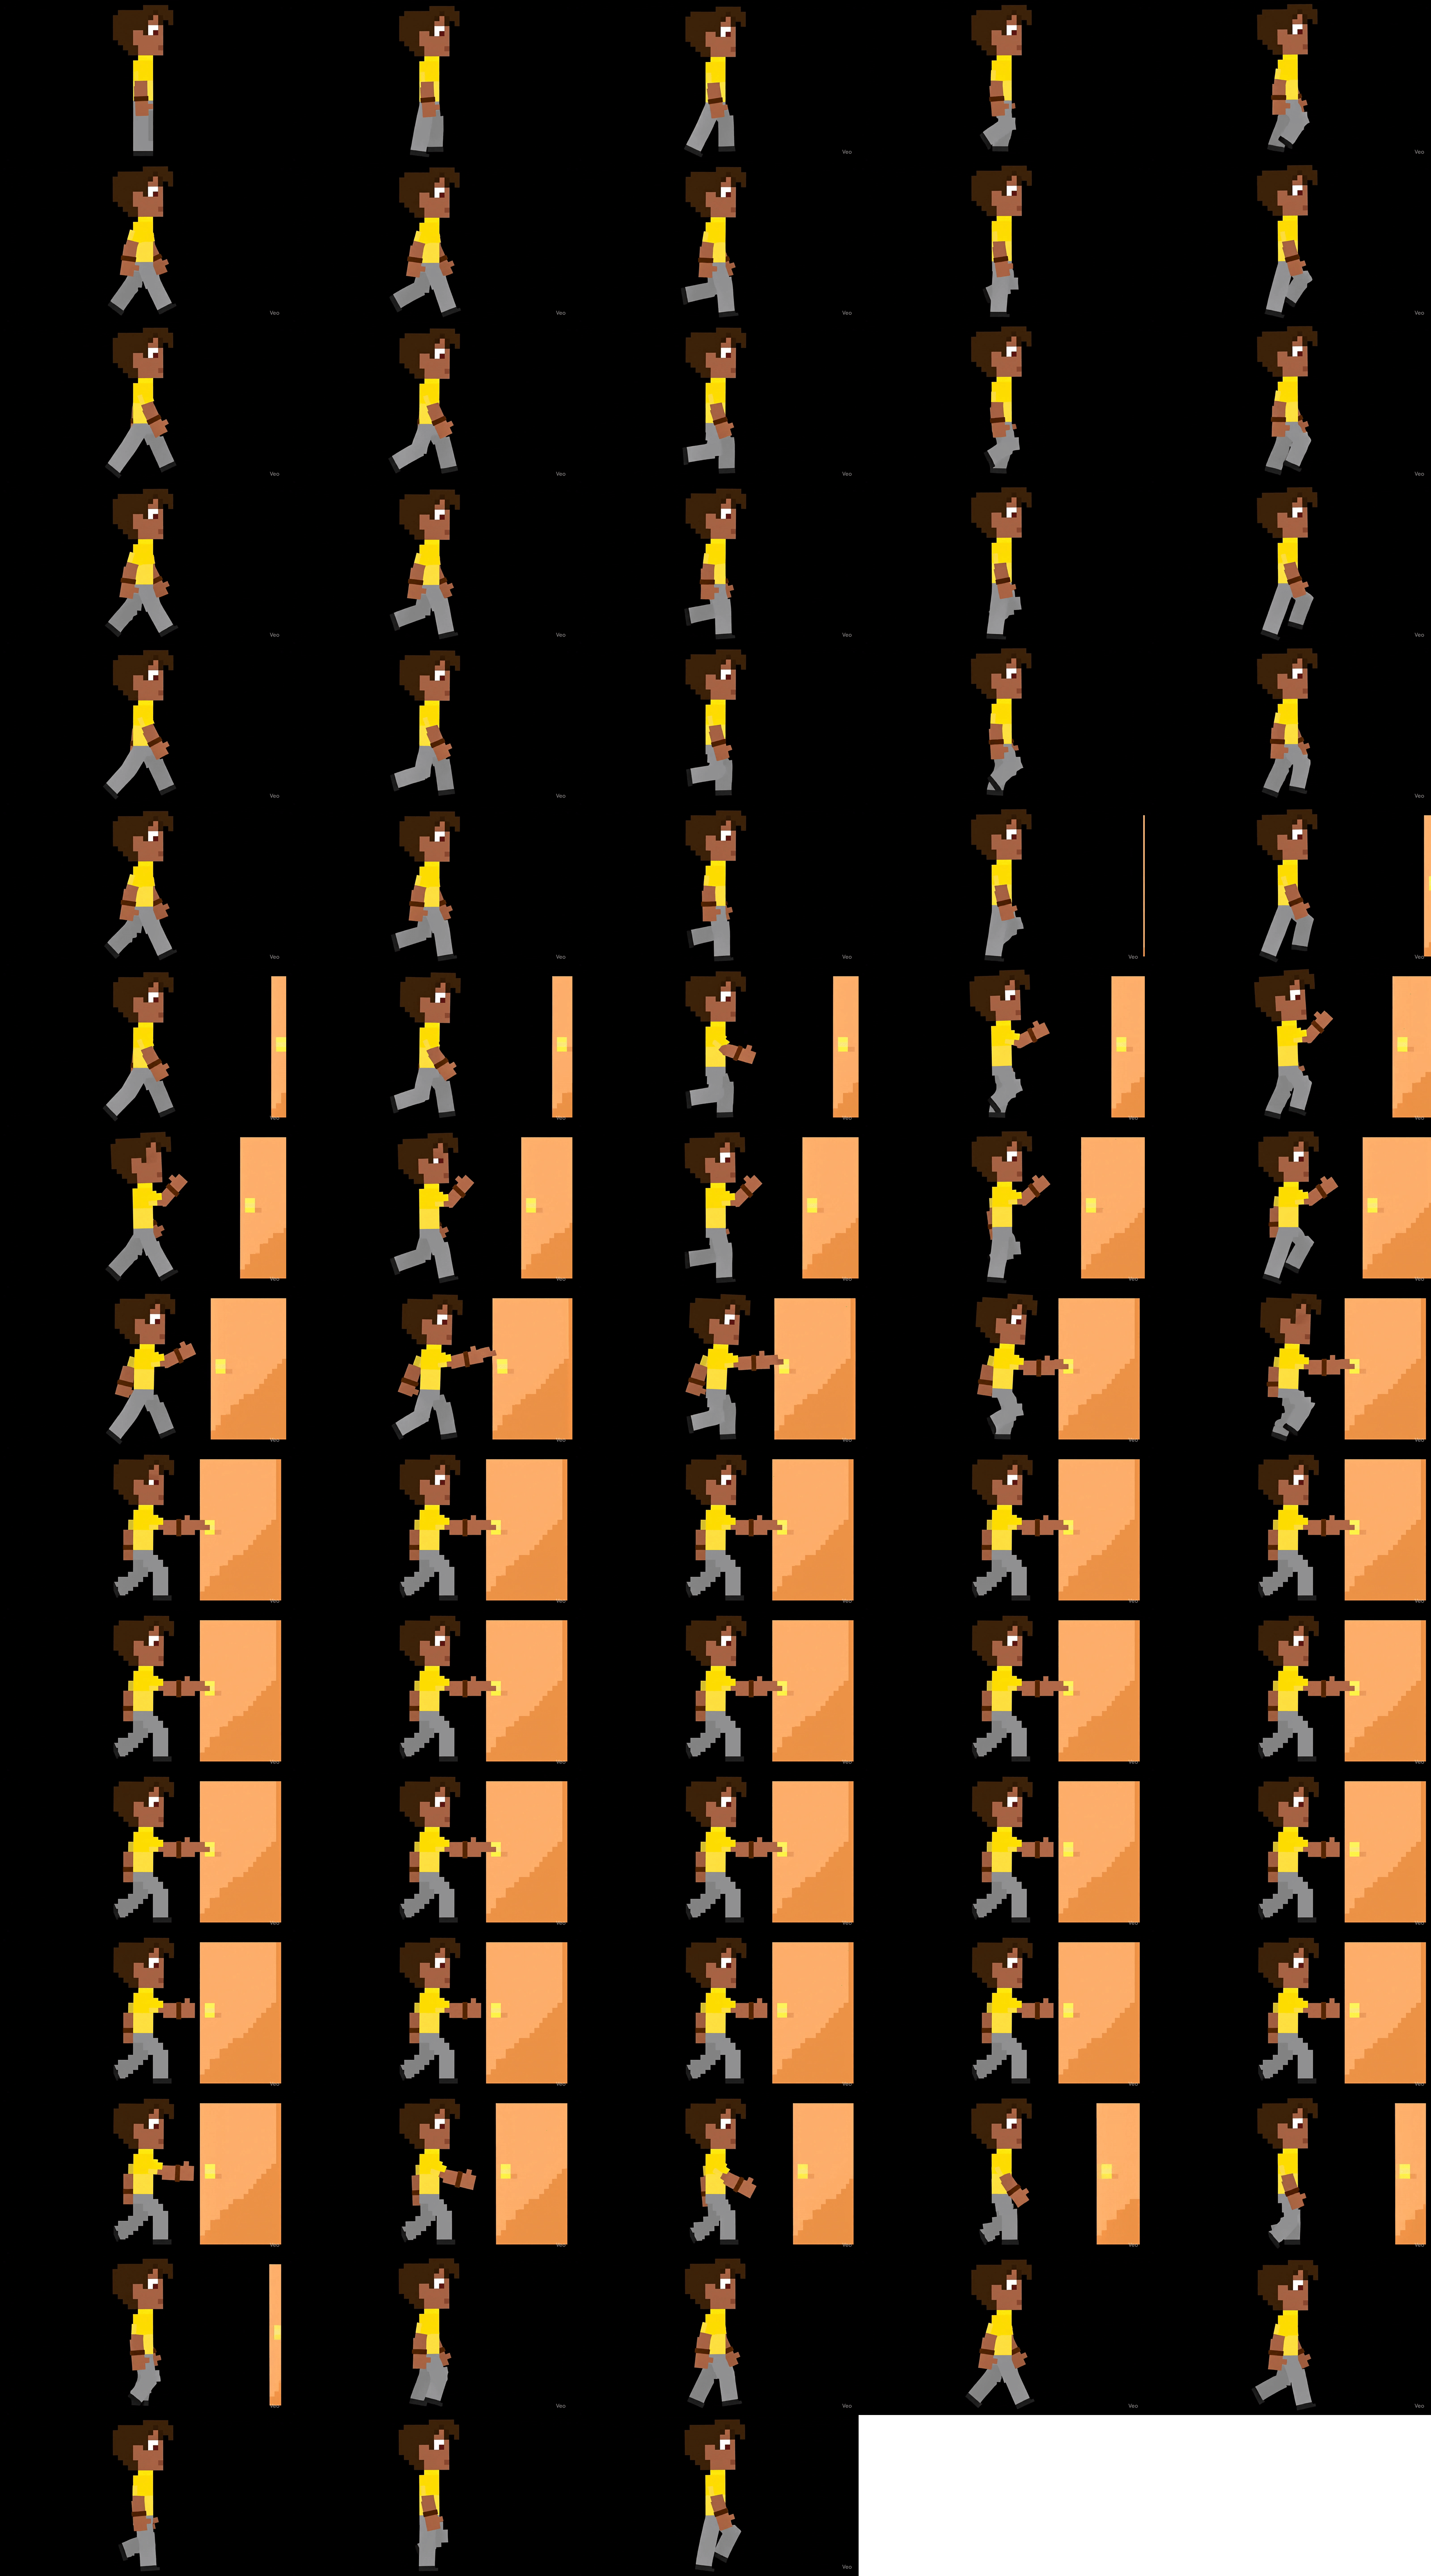
\includegraphics[width=0.6\linewidth]{figs/geminiPro/sprite sheet/video6.png}
    \legend{\small Fonte: Elaborada pela autora, utilizando a ferramenta ezgif.}
\end{figure}

\begin{figure}[htbp]
    \centering
    \caption{\small Imagem após remoção do trecho onde a porta aparece}
    \label{fig:geminiProAbrirPortaCorte}
    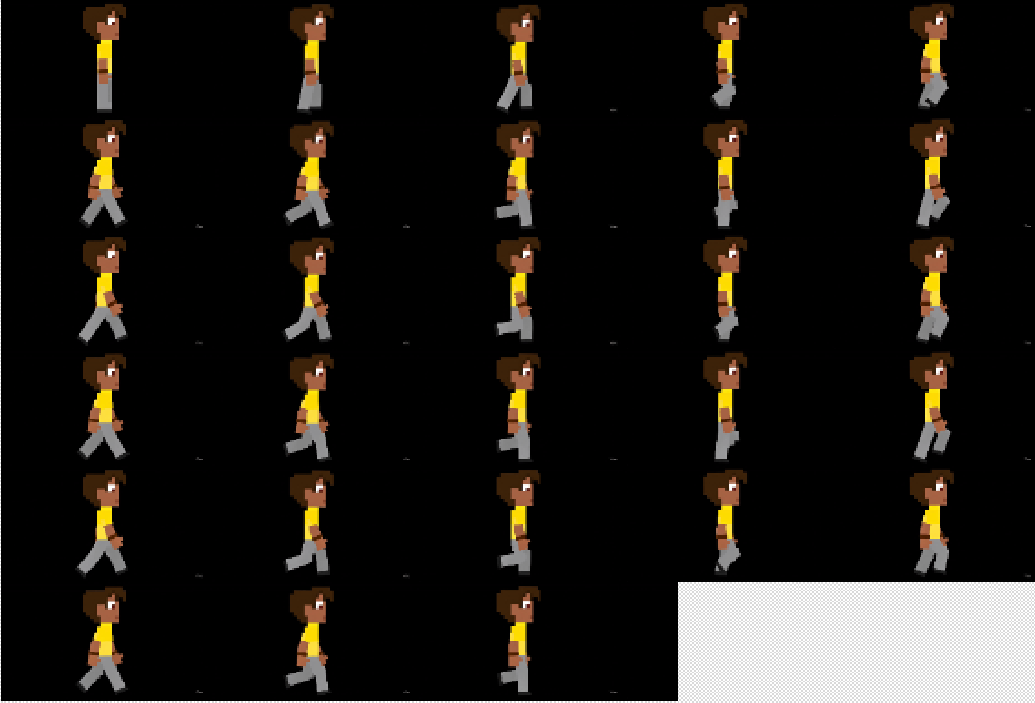
\includegraphics[width=0.7\linewidth]{figs/geminiPro/sprite sheet/walking_grande.PNG}
    \legend{\small Fonte: Elaborada pela autora, utilizando a ferramenta Pixilart.}
\end{figure}

\begin{figure}[htbp]
    \centering
    \caption{\small Imagem após ajuste do tamanho dos pixels}
    \label{fig:geminiProAbrirPortaPixel}
    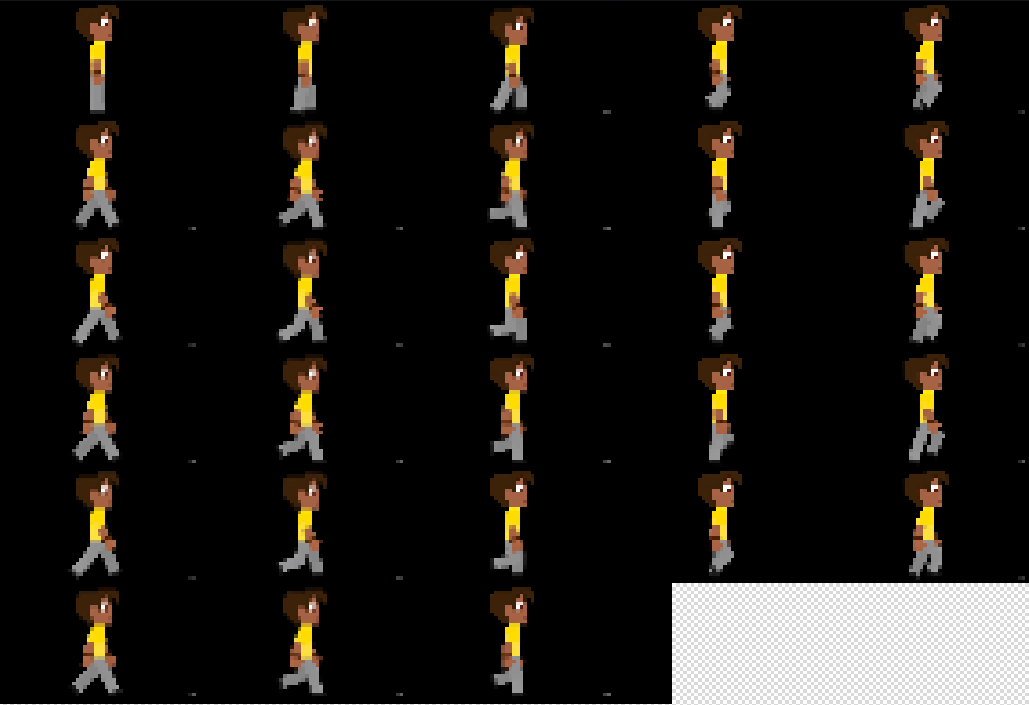
\includegraphics[width=0.7\linewidth]{figs/geminiPro/sprite sheet/walking_ajustado.PNG}
    \legend{\small Fonte: Elaborada pela autora, utilizando a ferramenta Pixilart.}
\end{figure}

\begin{figure}[htbp]
    \centering
    \caption{\small Imagem após remoção do fundo}
    \label{fig:geminiProAbrirPortaSemFundo}
    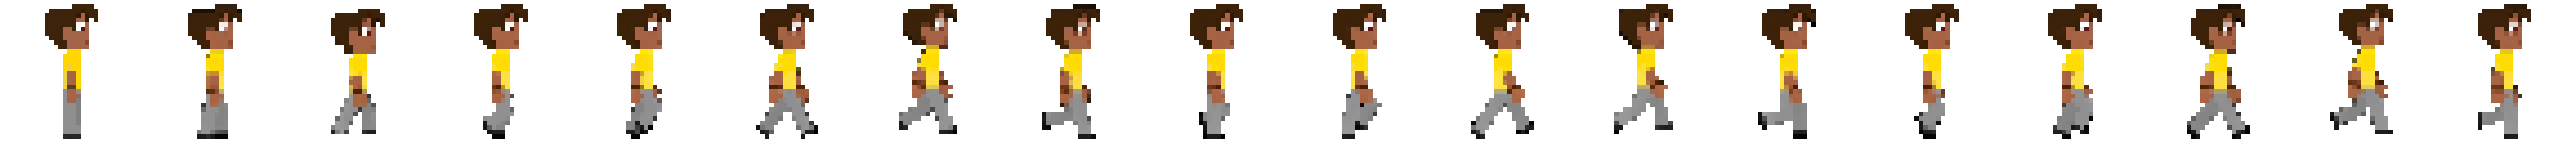
\includegraphics[width=1\linewidth]{figs/geminiPro/sprite sheet/walking_sprite_sheet_grande.png}
    \legend{\small Fonte: Elaborada pela autora, utilizando a ferramenta Pixilart.}
\end{figure}

